\chapter{Polinomios positivos y sumas de cuadrados}
%\noindent Referencia principal: \cite[Capítulo 3]{Lasserre2010}.

\section{Introducci\'on}


Notamos $\R[\xb] = \R[x_1, \dots, x_n]$ al anillo de polinomios sobre $\R$ en $n$ variables.

Dado un polinomio $p(\xb) \in \R[\xb]$, decimos que
\begin{itemize}
\item $p$ es \emph{positivo} ($p \ge 0$) si $p(\xb) \ge 0$ para todo $\xb \in \R^n$ (y \emph{estrictamente positivo} si $p > 0$ para todo $\xb \in \R^n$).
\item $p$ es una \emph{suma de cuadrados} (SOS) si existen $q_1, \dots, q_s \in \R[\xb]$ tales que
$$
p = q_1^2 + \dots + q_s^2.
$$
\end{itemize}

\begin{prop}
Si $p$ es SOS entonces $p \ge 0$.
\end{prop}

\begin{problem}
Dado un polinomio $p(\xb) \in \R[\xb]$, determinar si se puede escribir como suma de cuadrados (SOS) $p = p_1^2 + \dots + p_s^2$ y construir la descomposici\'on (aproximada o exacta).
\end{problem}

Algunas aplicaciones de sumas de cuadrados son:
\begin{itemize}
\item certificados de positividad,
\item La ecuación $p(\xb) + 1 = 0$ no tiene soluciones reales si $p$ es una suma de cuadrados,
\item Dado un polinomio $p$, si queremos hallar el mínimo de $p$ en $S = \R^n$ o en una regi\'on $S = \{ \xb \in \R^n : g(\xb) \ge 0\}$, para polinomios $\{g_1, \dots, g_s\}$, tenemos
\[
\min\{f(x) : \xb \in S\} = \sup\{a \in \R | f - a \ge 0 \text{ en } S\}.
\]
\end{itemize}


\section{Sumas de cuadrados en una variable}

\begin{proposition}
Si $p \in \R[x]$ (polinomios en una variable) entonces
$$
p \text{ es suma de cuadrados } \iff p \text{ es positivo}
$$
\end{proposition}

\begin{proof}
Tomamos $p \ge 0$. Por el teorema fundamental del \'algebra, podemos factorizar
\[
p(x) = \prod_{i=1}^r (x-a_i) \prod_{j=1}^t (x-b_j)(x - \bar b_j),
\]
donde $a_i \in \R$ son las raíces reales y $b_j, \bar b_j \in \C \smallsetminus \R$ son las raíces complejas conjugadas.

Si la multiplicidad de alguna raíz real $a$ es impar, entonces $p$ atraviesa transversalmente al eje $X$ en $a$ y por lo tanto no puede ser $p \ge 0$.

Por lo tanto, todas las raíces reales aparecen con multiplicidad par y podemos factorizar
\[
p(x) = \prod_{i=1}^s (x-a_i)^{2k_i} \prod_{j=1}^t (x-b_j)(x - \bar b_j).
\]

Para las raíces complejas tenemos
\begin{align*}
(x-b_j)(x - \bar b_j) &= (x - (\alpha_i + I \beta_i  ))(x - (\alpha_i - I  \beta_i )) \\
&= ((x - \alpha_i) - I\beta_i  ))((x - \alpha_i) + I \beta_i  )) \\
&= (x - \alpha_i)^2 + \beta_i^2,
\end{align*}
que es una suma de cuadrados.

Concluimos que $p(x)$ es un producto de sumas de cuadrados, y por lo tanto, distribuyendo los productos, $p(x)$ es una suma de cuadrados.

Más aún, utilizando la identidad
\[
(a^2+b^2)(c^2+d^2) = (ac+bd)^2 + (ad-bc)^2
\]
podemos escribir a cualquier polinomio $p(x) \ge 0$ como suma de 2 cuadrados.

\end{proof}


\section{Sumas de cuadrados en varias variables}

\begin{prop}
El polinomio
\[
f(x, y) = x^4y^2 + x^2y^4 - 3x^2y^2+1
 \]
 es no-negativo en $\R^2$ pero no puede escribirse como suma de cuadrados. (Motzkin, 1967)
\end{prop}

\begin{proof}
Veamos primero $f \ge 0$. Por la desigualdad aritmética-geométrica,
$$
\frac{x^4y^2 + x^2y^4 + 1}{3} \ge \sqrt[3]{(x^4y^2)(x^2y^4) 1} = \sqrt[3]{x^6y^6} = x^2y^2,
$$
y despejando obtenemos $x^4y^2 + x^2y^4 - 3x^2y^2+1 \ge 0$

Para ver que el polinomio de Motzkin no es una suma de cuadrados, 
escribimos $f = p_1^2 + \dots + p_s^2$, $p_i \in \R[x, y, z_1, ...,z_m]$. Vamos obteniendo condiciones sobre los posibles polinomios que pueden aparecer en la descomposición.

\begin{enumerate}
\item Podemos evaluar $z_i=0$ para todo $i$ y obtenemos una descomposición en $\R[x, y]$.
\item Si tomamos un monomio $m$ en los $p_i$ con el mayor grado $d$ en $x$, el monomio $m^2$ no se va a cancelar en la suma, y por lo tanto debe ser un monomio de $f$.
\item Por lo tanto, debe ser $d \le 2$.
\item Luego, siguiendo el mismo razonamiento, no puede aparecer $x^2y^2$ en ningún $p_i$.
\item Luego, tampoco pueden aparecer $x^2$ ni $y^2$ en ningún $p_i$.
\item Finalmente, no puede aparecer $x$ ni $y$ en ningún $p_i$.
\item Concluimos que los polinomios $p_i$ son de la forma
$$
a x^2y + b x y^2 + c xy + d,
$$
con $a, b, c, d \in \R$.
\item Al elevar al cuadrado un polinomio de esta forma, el coeficiente de $x^2y^2$ es siempre no-negativo. ¡Absurdo!
\end{enumerate}

\end{proof}

%------------------------------------------------------------------

Podemos extender el razonamiento anterior a casos más generales. Comenzamos realizando algunas definiciones.

\begin{definition}
Dado un vector $\ab \in \N_0^n$, $\ab = (a_1, \dots, a_n)$, definimos el monomio $m = \xb^{\ab}$ como
$$
\xb^{\ab} = x_1^{a_1} x_2^{a_2} \cdots x_n^{a_n},
$$
y análogamente, para un monomio $m$ de esa forma, llamamos a $\ab = (a_1, \dots, a_n) \in \R^n$ su \emph{vector de exponentes}.
\end{definition}

\begin{definition}
Dado un polinomio $p \in \K[\xb]$, definimos el \emph{soporte} de $p$, $\supp(p)$, como el conjunto de todos los vectores de exponentes de los monomios que aparecen en $p$.

Definimos  su \emph{polítopo de Newton} $\mathcal{N}(p)$ como la cápsula convexa de los vectores de exponentes de los monomios que aparecen en $p$,
$$
\mathcal{N}(p) = \conv(\supp(p)).
$$
\end{definition}

Por ejemplo, si $p = x_1 x_2^2 + x_2^2 + x_1 x_2 x_3$ entonces
$$
\mathcal{N}(p) = \conv{(\{(1,2,0), (0,2,0), (1,1,1)\})},
$$
que es un triángulo en $\R^3$.

Utilizando el polítopo de Newton podemos obtener información sobre los monomios que pueden aparecer en una suma de cuadrados.

\begin{theorem}
Si $p = \sum_{i = 1}^s q_i^2$ es una suma de cuadrados, entonces
$$
\mathcal{N}(q_i) \subset \frac{1}{2}\mathcal{N}(p).
$$
\end{theorem}

\begin{proof}
Consideramos la cápsula convexa de la unión de todos los polítopos de Newton de los $q_i$, $1 \le i \le s$,
$$
K = \conv(\cup_{i=1}^s\mathcal{N}(q_i)).
$$

Recordamos que un polítopo está generado por las combinaciones convexas de sus vértices.

Tomamos un \emph{vértice} $\vb$ de $K$ y suponemos por contradicción que $2\vb \not\in \supp(p)$.

Si $\alpha \xb^{\vb}$ aparece en $q_i$, entonces $\alpha^2 \xb^{2\vb}$ aparece en $q_i^2$ con coeficiente $\alpha^2 > 0$. Para que estos términos se cancelen, debe aparecer también $\xb^{2\vb}$ como producto cruzado de términos de algunos $q_i$.

Es decir, existen $\ub, \wb \in K$ tales que $2\vb = \ub+\wb$.

Pero luego, $\vb = \frac{\ub+\wb}{2} \in K$ no es un vértice, lo que contradice la hipótesis.

Concluimos que para cualquier vértice $\vb$ de $K$, $2\vb \in \supp(p) \subset \mathcal{N}(p)$.

Como $2K$ es un polítopo, es la cápsula convexa del conjunto de todos sus vértices.

Como todos los vértices de $2K$ están contenidos en el conjunto convexo $\mathcal{N}(p)$, obtenemos $2K \subset \mathcal{N}(p)$.

Por lo tanto, $2 \mathcal{N}(q_i) \subset \mathcal{N}(p)$ para todo $1 \le i \le n$.

\end{proof}

\textbf{Motzkin revisitado}

Utilizando este resultado podemos simplificar la demostración de que el polinomio de Motzkin $f(x, y) = x^4y^2 + x^2y^4 - 3x^2y^2+1$ no es una suma de cuadrados.

A la izquierda representamos el polítopo de Newton $\mathcal{N}(f)$ y a la derecha $\frac{1}{2}\mathcal{N}(f)$.

\begin{figure}
    \centering
    \begin{minipage}{0.45\textwidth}
        \centering
        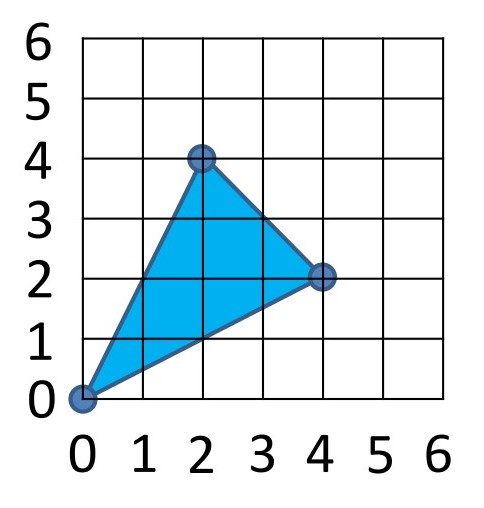
\includegraphics[width=0.5\textwidth]{sos_motzkinHull-2.jpg} % first figure itself
        %\caption{first figure}
    \end{minipage}\hfill
    \begin{minipage}{0.45\textwidth}
        \centering
        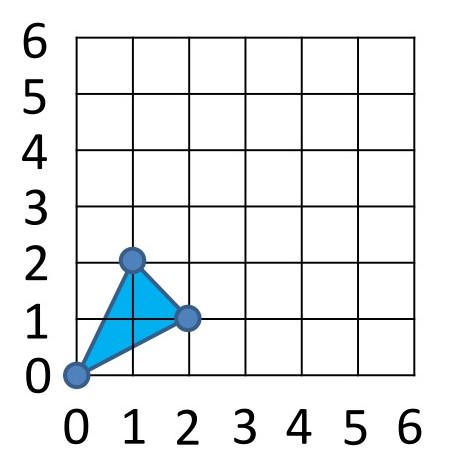
\includegraphics[width=0.5\textwidth]{sos_motzkinHull-3.jpg} % second figure itself
        %\caption{second figure}
    \end{minipage}
\end{figure}

Concluimos inmediatamente que $f = \sum_{i=1}^s q_i$, los $q_i$ son de la forma
$$
q_i(x, y) = a x^2y + b x y^2 + c xy + d.
$$


\textbf{Grado de un polinomio}

Definimos el grado de un monomio $x_1^{a_1} \cdots x_n^{a_n}$ como
$$d = |\ab| = a_1 + \dots + a_n,$$
y el grado de un polinomio $p \in \R[\xb]$ como el mayor de los grados de sus monomios.


\textbf{Polinomios homogéneos}

Decimos que un polinomios es homogéneo si todos sus monomios tienen el mismo grado.

Dado un polinomio no-homogéneo $f(x_1, \dots, x_n)$ de grado $d$, definimos su homogeneización
$$F(x_0, x_1, \dots, x_n) = x_0^d f\left(\frac{x_1}{x_0}, \dots, \frac{x_n}{x_0}\right)$$
que equivale a multiplicar cada monomio por la potencia de $x_0$ apropiada para que todos los términos tengan grado $d$.


Por ejemplo, homegeneizamos $f(x_1, x_2) = x_1^4x_2^2 + x_1^2x_2^4 - 3x_1^2x_2^2+1$ a
$$
F(x_0, x_1, x_2) = x_1^4x_2^2 + x_1^2x_2^4 - 3x_0^2x_1^2x_2^2+x_0^6
$$
multiplicando cada término por la potencia de $x_0$ apropiada.

Como corolario del teorema anterior sobre los polítopos de Newton, obtenemos el siguiente resultado.

\begin{prop} Si $p(\xb)$ es SOS homogéneo, entonces $p(\xb)$ tiene grado par $2d$ y es suma de cuadrados de polinomios homogéneos de grado $d$.
\end{prop}

\begin{prop} Las condiciones de no-negatividad y suma de cuadrados se mantienen al homogeneizar, por lo tanto no perdemos generalidad al asumir polinomios homogéneos.
\end{prop}

Vamos a trabajar a partir de ahora con polinomios homogéneos.

\textbf{Los conos de polinomios positivos y sumas de cuadrados}

Llamamos
\begin{itemize}
\item $H_{n,2d}$ al espacio vectorial de polinomios homog\'eneos de $n$ variables y grado $2d$.
\item $P_{n,2d} \subset H_{n,2d}$ al conjunto de polinomios homog\'eneos positivos de $n$ variables y grado $2d$.
\item $\Sigma_{n,2d} \subset P_{n,2d}$ al subconjunto de sumas de cuadrados.
\end{itemize}

\begin{prop}
$P_{n,2d}$ y $\Sigma_{n,2d}$ son conos convexos cerrados de dimensión máxima.
\end{prop}

\begin{ejercicio}
Demostrar que $P_{n,2d}$ es cerrado escribiéndolo como intersección de infinitos semi-espacios cerrados.
\end{ejercicio}

\section{El teorema de Hilbert}

\begin{theorem}[Teorema de Hilbert (1888)]
Los conjuntos $P_{n,2d}$ y $\Sigma_{n,2d}$ son iguales solo en los siguientes casos:

\begin{enumerate}
 \item $n = 2$
 \item $2d=2$
 \item $(n,2d) = (3,4)$
\end{enumerate}
\end{theorem}

\section{Problema de programaci\'on semidefinida}
Dado $p \in \R[x_1, \dots, x_n]$, homog\'eneo de grado $2d$, podemos escribirlo como un producto
\[
p(\xb) = \vb(\xb)^T \Qb \vb(\xb),
\]
con $\vb$ el vector de monomios de grado $d$ y $\Qb \in \R^{M(d) \times M(d)}$ sim\'etrica, con $M(d) =  \binom{n+d-1}{d}$, la cantidad de monomios de grado $d$ en $n$ variables

Esta ecuación nos una ecuación lineal para cada coeficiente de $p$, en total $\binom{n+2d-1}{2d}$ ecuaciones.

\begin{example}
Para el polinomio $p(x,y) = 10x^4+2x^3y+27x^2y^2-24xy^3+5y^4$, planteamos la ecuación matricial
$10x^4+2x^3y+27x^2y^2-24xy^3+5y^4 = $
\[
\begin{pmatrix}
x^2 & xy & y^2
\end{pmatrix}
\begin{pmatrix}
q_{00} & q_{10} & q_{20} \\
q_{10} & q_{11} & q_{21} \\
q_{20} & q_{21} & q_{22} \\
\end{pmatrix}
\begin{pmatrix}
x^2 \\
xy \\
y^2 \\
\end{pmatrix}
\]
y obtenemos que se debe cumplir la igualdad
\begin{align*}
& 10x^4+2x^3y+27x^2y^2-24xy^3+5y^4 = \\
= \  & q_{00} x^4 + 2q_{10} x^3y + (2q_{20} + q_{11})x^2y^2 + 2q_{21}xy^3 + q_{22} y^4.
\end{align*}


Igualando coeficiente a coeficiente
\begin{align*}
& 10x^4+2x^3y+27x^2y^2-24xy^3+5y^4 = \\
= \  & q_{00} x^4 + 2q_{10} x^3y + (2q_{20} + q_{11})x^2y^2 + 2q_{21}xy^3 + q_{22} y^4
\end{align*}
obtenemos
\begin{align*}
q_{00} &= 10 \\
2q_{10} &= 2 \\
2q_{20} + q_{11} &= 27 \\
2q_{21} &= -24 \\
q_{22} &= 5
\end{align*}

Despejando, obtenemos

$10x^4+2x^3y+27x^2y^2-24xy^3+5y^4 = $
\[
\begin{pmatrix}
x^2 & xy & y^2
\end{pmatrix}
\begin{pmatrix}
10 & 1 & a \\
1 & -2a + 27 & -12 \\
a & -12 & 5 \\
\end{pmatrix}
\begin{pmatrix}
x^2 \\
xy \\
y^2 \\
\end{pmatrix}
\]
para cualquier $a \in \R$, y todas las matrices que cumplen la igualdad son de esta forma.


\textbf{Descomposición como combinación lineal de cuadrados}

Tomamos por ejemplo $a = 1$ y diagonalizamos (descomposici\'on $LDL^t$ por eliminaci\'on gaussiana):
{\scriptsize
\[
\begin{pmatrix}
10 & 1 & 1 \\
1 & 25 & -12 \\
1 & -12 & 5 \\
\end{pmatrix}
=
\begin{pmatrix}
1 & 0 & 0 \\
\frac{1}{10} & 1 & 0 \\
\frac{1}{10} & -\frac{121}{249} & 1 \\
\end{pmatrix}
\begin{pmatrix}
10 & 0 & 0 \\
0 & \frac{249}{10} & 0 \\
0 & 0 & -\frac{244}{249} \\
\end{pmatrix}
\begin{pmatrix}
1 & \frac{1}{10}  & \frac{1}{10}  \\
0 & 1 & -\frac{121}{249}  \\
0 & 0 & 1 \\
\end{pmatrix}
\]
}

Obtenemos la descomposici\'on
\[
f = 10\left(x^2+\frac{1}{10}xy+\frac{1}{10}y^2\right)^2 + \frac{249}{10}\left(xy-\frac{121}{249}y^2\right)^2 - \frac{244}{249}\left(y^2\right)^2
\]

No es una suma de cuadrados porque el último coeficiente es negativo.

\end{example}

\textbf{Signatura y suma de cuadrados}

La cantidad de valores positivos en la diagonal es igual a la cantidad de autovalores positivos.
Por lo tanto, debemos hallar $a \in \R$ tal que $\Qb$ sea semidefinida positiva $\longrightarrow$ \emph{Problema de programaci\'on semidefinida}.

Concretamente, tenemos el siguiente resultado.

\begin{prop} Si $p(\xb) \in \R[\xb]$ es un polinomio homogéneo de grado $2d$, las siguientes propiedades son equivalentes:
\begin{enumerate}
\item $p(\xb)$ es una suma de cuadrados,
\item existe $\Qb \succeq 0$ que satisface la fórmula $p(\xb) = \vb(\xb)^T \Qb \vb(\xb)$,
\end{enumerate}
para $\vb(\xb)$ el vector de monomios de grado $d$ en $\R[\xb]$.
\end{prop}

\begin{proof}

Para probar (2) $\Rightarrow$ (1), dada una matriz $\Qb \succeq 0$, podemos factorizarla $\Qb = \Lb^T \Lb$, con $\Lb$ triangular inferior y obtenemos
$$
p(\xb) = \vb(\xb)^T \Qb \vb(\xb) = \vb(\xb)^T \Lb^T \Lb \vb(\xb) = \sum (\inner{\Lb_i}{\vb(\xb)})^2 = \sum q_i(\xb)^2.
$$

Recíprocamente, si $p(\xb)$ es SOS, $p(\xb) = \sum q_i(\xb)^2$, construimos la matriz $\Xb$ tomando en la fila $i$ los coeficientes de $q_i(\xb)$ y tomamos $\Qb = \Xb^T \Xb \succeq 0$.

\end{proof}

\textbf{Representación núcleo y representación imagen}

Vemos que podemos plantear el problema mediante ecuaciones sobre los coeficientes de $\Qb$, que se obtienen igualando coeficiente a coeficiente la expresión
$$p(\xb) = \vb(\xb)^T \Qb \vb(\xb).$$
Llamamos representación núcleo o implícita a esta representación.

Resolviendo las ecuaciones, podemos plantear el problema mediante una desigualdad lineal matricial (LMI)
$$\Qb = \Ab_0 + \sum_i y_i \Ab_i$$
que llamamos representación imagen o explícita.


Pregunta: ¿para el ejemplo anterior cuál es la representación explícita y cuál es la representación implícita?


\section{Programas Sumas de Cuadrados}

\subsection{Motivación}

Vimos la siguiente aplicación de polinomios no-negativos:

Dado un polinomio $p$, si queremos hallar el mínimo de $p$ en $S = \R^n$, planteamos
\[
\min\{f(\xb) : \xb \in \R^n\} = \sup\{\gamma \in \R | f(\xb) - \gamma \ge 0 \ \forall \xb \in \R^n\}.
\]

Para $\gamma \in \R$ dado, podemos reemplazar la condición $f(\xb) - \gamma \ge 0$ por $f(\xb)$ es SOS, lo que nos da un problema de factibilidad de un SDP.

Resolviendo estos problemas para distintos valores de $\gamma$, podemos obtener cotas para el mínimo de $p$.

Pregunta: ¿podemos obtener la mejor cota resolviendo un solo problema SDP?


Vimos cómo verificar si un polinomio dado es una suma de cuadrados.

Podemos extender los resultados para definir una clase de problemas de optimización convexa que llamamos \emph{programas sumas de cuadrados} (SOS).

\begin{definition}
Un problema de optimización por sumas de cuadrados o programa SOS es un problema de optimización convexa de la forma
\begin{alignat*}{2}
  & \text{maximizar: } & & b_1 y_1 + \dots + b_m y_m  \\
   & \text{sujeto a: } & \quad & p_i(\xb; \yb) \text{ es SOS }, 1 \le i \le k,
\end{alignat*}
donde $\yb = (y_1, \dots, y_m) \in \R^m$ es la variable de optimización, $b_i \in \R$, $1 \le i \le m$, $p_i(\xb; \yb) = a_{i0}(\xb) + a_{i1}(\xb) y_1 + \dots + a_{im}(\xb) y_m$, $1 \le i \le k$ y $a_{ij}(\xb) \in \R[\xb]$ son polinomios dados.
\end{definition}

\textbf{Observaciones:}
\begin{itemize}
\item Los polinomios $p_i(\xb, \yb)$ son polinomios arbitrarios que son combinaciones afines en los parámetros $y_1, \dots, y_m$.
\item Las variables $\xb$ son variables ``dummy'', no optimizamos sobre ellas sino que son las indeterminadas de los polinomios $p_i$.
\end{itemize}

\textbf{Ejemplo.}
Consideramos el problema
\begin{alignat*}{2}
  & \text{maximizar: } & & y_1 + y_2  \\
  & \text{sujeto a: } & \quad & x^4 + y_1 x + (2 + y_2) \quad \text{es SOS,} \\
  &  & \quad & (y_1 - y_2 + 1)x^2 + y_2 x + 1 \quad  \text{es SOS.}
\end{alignat*}


Aunque a primera vista, los programas SOS parecen más generales que los problemas SDP, cada restricción del problema podemos plantearla como la existencia de una matriz $\Qb_i \succeq 0$ tal que
$$
p_i(\xb; \yb) = \vb^T \Qb_i \vb,
$$
donde las coordenadas de $\Qb_i$ dependen linealmente de las variables $y_i$, $1 \le i \le m$, y por lo tanto un programa SOS es un problema SDP.


\begin{example}
Para la restricción
$$p_1(x; y_1, y_2) = x^4 + y_1 x + (2+y_2) \quad \text{ es sos }
$$
planteamos
$$
x^4 + y_1 x + (2+y_2) = \begin{pmatrix} 1 & x & x^2 \end{pmatrix}
\begin{pmatrix}
q_{00} & q_{10} & q_{20} \\
q_{10} & q_{11} & q_{21} \\
q_{20} & q_{21} & q_{22} \\
\end{pmatrix}
\begin{pmatrix} 1 \\ x \\ x^2 \end{pmatrix}
$$
y obtenemos la restricción $\Qb =
\begin{pmatrix}
2+y_2 & \frac{y_1}{2} & -\frac{a}{2} \\
\frac{y_1}{2} & a & 0 \\
-\frac{a}{2} & 0 & 1
\end{pmatrix} \succeq 0,
$ donde $a, y_1, y_2$ son las variables del problema SDP.
\end{example}

\subsection{Aplicación: optimización polinomial sin restricciones}

\textbf{Caso polinomios univariados}

Para encontrar el mínimo de un polinomio en una variable, utilizamos la equivalencia $
p(x) \ge \gamma \ \forall x \in \R \quad \iff \quad p(x) - \gamma \ge 0 \ \forall x \in \R$.

Obtenemos el siguiente problema de optimización:
\begin{alignat*}{2}
  & \text{maximizar: } & & \gamma  \\
  & \text{sujeto a: } & \quad & p(x) - \gamma \ge 0 \ \forall x \in \R.
\end{alignat*}

Como en una variable un polinomio es no-negativo si y solo si es SOS, obtenemos el problema SOS equivalente
\begin{alignat*}{2}
  & \text{maximizar: } & & \gamma  \\
  & \text{sujeto a: } & \quad & p(x) - \gamma \quad \text{es SOS}.
\end{alignat*}

\textbf{Caso polinomios multivariados}

Análogamente, si queremos encontrar el mínimo de un polinomio multivariado planteamos el problema de optimización:
\begin{alignat*}{2}
  & \text{maximizar: } & & \gamma  \\
  & \text{sujeto a: } & \quad & p(\xb) - \gamma \ge 0 \ \forall \xb \in \R^n.
\end{alignat*}

En el caso general este problema no se puede plantear eficientemente, pero podemos plantear el problema alternativo
\begin{alignat*}{2}
  & \text{maximizar: } & & \gamma  \\
  & \text{sujeto a: } & \quad & p(\xb) - \gamma \quad \text{es SOS}.
\end{alignat*}

Llamamos $p_{\star}$ al ínfimo de $p$ (que coincide con el óptimo del primer problema) y $p_{SOS}$ al óptimo del segundo problema.

Como el conjunto factible del problema SOS está incluido en el conjunto factible del primero, obtenemos la desigualdad
$$
p_{SOS} \le p_{\star}.
$$

Si bien en muchos casos (especialmente en dimensión baja) ambos óptimos coinciden, el primer problema es NP-hard y por lo tanto no podemos esperar que los óptimos coincidan siempre.


